\documentclass[12pt,a4paper]{article}

% ─── Page Layout ───────────────────────────────────────────────────────────────
\usepackage[a4paper, margin=0.8in, headheight=14pt]{geometry}

% ─── Fonts (XeLaTeX) ───────────────────────────────────────────────────────────
\usepackage{fontspec}
\usepackage{unicode-math}
\setmainfont{TeX Gyre Pagella}
\setmonofont[Scale=0.88]{TeX Gyre Cursor}
\setmathfont{Latin Modern Math}

% ─── Packages ──────────────────────────────────────────────────────────────────
\usepackage{xcolor}
\usepackage{colortbl}
\usepackage{titlesec}
\usepackage{enumitem}
\usepackage{tabularx}
\usepackage{booktabs}
\usepackage{array}
\usepackage{amsmath}
\usepackage{tikz}
\usetikzlibrary{shapes.geometric, arrows.meta, positioning, calc, fit, decorations.pathreplacing}
\usepackage{tcolorbox}
\tcbuselibrary{skins, breakable}
\usepackage{hyperref}
\usepackage{fancyhdr}
\usepackage{graphicx}
\usepackage{microtype}
\hyphenpenalty=10000
\exhyphenpenalty=10000
\sloppy
\usepackage{caption}
\usepackage{setspace}
\usepackage{multirow}
\usepackage{tocloft}

% ─── Q&A helper ────────────────────────────────────────────────────────────────
\newcommand{\Q}[1]{\textbf{#1}\par\noindent\ignorespaces}

% ─── Colour Palette ────────────────────────────────────────────────────────────
\definecolor{myred}{RGB}{196,30,58}
\definecolor{mydark}{RGB}{30,30,50}
\definecolor{mygreen}{RGB}{14,120,80}
\definecolor{myteal}{RGB}{0,130,140}
\definecolor{myamber}{RGB}{180,100,0}
\definecolor{mypurple}{RGB}{100,30,160}
\definecolor{mygray}{RGB}{246,247,249}
\definecolor{mgframe}{RGB}{180,185,200}
\definecolor{watermark}{RGB}{145,150,170}
\definecolor{hdrred}{RGB}{250,232,235}
\definecolor{hdrgreen}{RGB}{220,244,233}
\definecolor{hdrteal}{RGB}{220,242,244}
\definecolor{hdramber}{RGB}{253,242,215}
\definecolor{hdrpurple}{RGB}{238,228,255}
\definecolor{hdrgray}{RGB}{238,240,245}
\definecolor{rowalt}{RGB}{250,251,253}

% ─── Section Formatting ────────────────────────────────────────────────────────
\titleformat{\section}
  {\large\bfseries\color{myred}}{\thesection.}{0.5em}{}
  [\vspace{1pt}{\color{myred}\rule{\linewidth}{0.8pt}}]
\titleformat{\subsection}
  {\normalsize\bfseries\color{myteal}}{\thesubsection}{0.5em}{}
\titlespacing*{\section}{0pt}{18pt}{7pt}
\titlespacing*{\subsection}{0pt}{11pt}{4pt}

% ─── Paragraph ─────────────────────────────────────────────────────────────────
\setlength{\parindent}{0pt}
\setlength{\parskip}{4pt}

% ─── TOC Styling ───────────────────────────────────────────────────────────────
\renewcommand{\cfttoctitlefont}{\large\bfseries\color{myred}}
\renewcommand{\cftaftertoctitle}{\par\noindent{\color{myred}\rule{\linewidth}{0.8pt}}}
\setlength{\cftbeforetoctitleskip}{0pt}
\setlength{\cftaftertoctitleskip}{6pt}
\renewcommand{\cftsecfont}{\normalsize\bfseries\color{mydark}}
\renewcommand{\cftsecpagefont}{\normalsize\bfseries\color{mydark}}
\renewcommand{\cftsecleader}{\cftdotfill{\cftdotsep}}
\setlength{\cftbeforesecskip}{7pt}
\renewcommand{\cftsubsecfont}{\small\color{mydark}}
\renewcommand{\cftsubsecpagefont}{\small\color{mydark}}
\setlength{\cftbeforesubsecskip}{3pt}
\setlength{\cftsubsecindent}{1.4em}

% ─── Table helpers ─────────────────────────────────────────────────────────────
\renewcommand{\arraystretch}{1.45}
\setlength{\tabcolsep}{6pt}
\arrayrulecolor{mydark}
\newcolumntype{B}[1]{>{\small\bfseries\raggedright\arraybackslash}m{#1}}
\newcolumntype{Y}{>{\small\raggedright\arraybackslash}X}
\renewcommand{\tabularxcolumn}[1]{m{#1}}

% ─── Header / Footer ───────────────────────────────────────────────────────────
\pagestyle{fancy}
\fancyhf{}
\fancyhead[L]{\small\color{myred}\textbf{PE-EC701A}\;\color{mydark}--- Microwave Theory and Technique}
\fancyhead[R]{\small\color{myteal}\textbf{Module 7 Notes}}
\fancyfoot[C]{\small\color{mydark}\thepage}
\fancyfoot[R]{\small\color{watermark}\textit{\copyright\ Biraj}}
\renewcommand{\headrulewidth}{0.5pt}
\renewcommand{\footrulewidth}{0.3pt}

% ─── Hyperref ──────────────────────────────────────────────────────────────────
\hypersetup{
  colorlinks=true, linkcolor=myteal, urlcolor=myteal,
  pdfauthor={Biraj Sarkar},
  pdftitle={PE-EC701A --- Module 7 Notes}
}

% ─── tcolorbox styles ──────────────────────────────────────────────────────────
\tcbset{
  tikzbox/.style={
    colback=mygray, colframe=mgframe, boxrule=0.6pt, arc=4pt,
    left=8pt, right=8pt, top=6pt, bottom=6pt,
    colbacktitle=mgframe, coltitle=mydark,
    fonttitle=\small\bfseries
  },
  defbox/.style={
    colback=hdrgreen, colframe=mygreen, boxrule=0.8pt, arc=4pt,
    left=9pt, right=9pt, top=6pt, bottom=6pt,
    colbacktitle=mygreen, coltitle=white,
    fonttitle=\small\bfseries
  },
  formulabox/.style={
    colback=hdrteal, colframe=myteal, boxrule=0.8pt, arc=4pt,
    left=9pt, right=9pt, top=7pt, bottom=7pt,
    colbacktitle=myteal, coltitle=white,
    fonttitle=\small\bfseries
  },
  examplebox/.style={
    colback=hdramber, colframe=myamber, boxrule=0.8pt, arc=4pt,
    left=9pt, right=9pt, top=6pt, bottom=6pt,
    colbacktitle=myamber, coltitle=white,
    fonttitle=\small\bfseries
  },
  masonbox/.style={
    colback=hdrpurple, colframe=mypurple, boxrule=0.8pt, arc=4pt,
    left=9pt, right=9pt, top=6pt, bottom=6pt,
    colbacktitle=mypurple, coltitle=white,
    fonttitle=\small\bfseries
  },
  exambox/.style={
    colback=hdrpurple, colframe=mypurple, boxrule=1pt, arc=5pt,
    left=10pt, right=10pt, top=8pt, bottom=8pt,
    colbacktitle=mypurple, coltitle=white,
    fonttitle=\bfseries,
    breakable, title after break={\textbf{Frequently Asked / Viva Questions (contd.)}}}
}
% Make all boxes breakable across pages
\tcbset{breakable}

% ─── TikZ styles ───────────────────────────────────────────────────────────────
\tikzset{
  block/.style={rectangle, draw=myteal, fill=hdrteal,
    text width=2.4cm, align=center, minimum height=0.95cm,
    font=\small, rounded corners=3pt, line width=0.7pt},
  redblock/.style={rectangle, draw=myred, fill=hdrred,
    text width=2.4cm, align=center, minimum height=0.95cm,
    font=\small, rounded corners=3pt, line width=0.7pt},
  netnode/.style={rectangle, draw=myteal, fill=hdrteal,
    text width=1.5cm, align=center, minimum height=0.8cm,
    font=\small, rounded corners=3pt, line width=0.7pt},
  sumjunc/.style={circle, draw=myamber, fill=hdramber,
    minimum size=0.62cm, font=\small, line width=0.8pt},
  snode/.style={circle, draw=mypurple, fill=hdrpurple,
    minimum size=0.55cm, font=\footnotesize, line width=0.7pt},
  arrow/.style={-Stealth, thick, color=mydark},
  redarrow/.style={-Stealth, thick, color=myred},
  line/.style={thick, color=mydark}
}

% ═══════════════════════════════════════════════════════════════════════════════
\begin{document}
% ═══════════════════════════════════════════════════════════════════════════════

\begin{center}
  {\LARGE\bfseries\color{myred} PE-EC701A --- Microwave Theory and Technique}\\[5pt]
  {\normalsize\color{mydark} Semester VII \quad$\bullet$\quad 3L:0T:0P \quad$\bullet$\quad 3 Credits}\\[3pt]
  {\normalsize\color{myteal}\textbf{Module 7 Exam Notes: Microwave Antennas}}\\[3pt]
  {\small\color{mydark} CGEC \;$|$\; B.Tech ECE (2023--27) \;$|$\; \textit{Biraj Sarkar}}
\end{center}
\vspace{2pt}
\noindent{\color{myred}\rule{\linewidth}{1.5pt}}
\vspace{2pt}

\hypersetup{linkcolor=mydark}
\tableofcontents
\hypersetup{linkcolor=myteal}
\newpage

% ===============================================================================
\section{Antenna Parameters}
% ===============================================================================

Antennas are transitions between guided waves and free-space radiation. They are characterized by several fundamental parameters.

\begin{tcolorbox}[defbox]
\textbf{Effective Aperture ($A_e$):} A parameter describing the power-collecting ability of an antenna. It is the ratio of received power to the incident wave power density:
\begin{equation}
  A_e = \frac{P_{\text{rec}}}{W_i} \quad (\text{m}^2)
\end{equation}
\end{tcolorbox}

\begin{tcolorbox}[formulabox, title={\textbf{Core Antenna Parameters}}]
\begin{enumerate}[label=\textbf{\arabic*.}, leftmargin=1.5em, itemsep=4pt, topsep=2pt]
  \item \textbf{Directive Gain ($G_d$) \& Directivity ($D$):} Directivity is the maximum value of directive gain in the peak radiation direction.
    \begin{equation}
      D = \frac{4\pi U_{\text{max}}}{P_{\text{rad}}}
    \end{equation}
  \item \textbf{Aperture Gain Relation:}
    \begin{equation}
      G = D \cdot \eta_{\text{rad}} = \frac{4\pi A_e}{\lambda^2}
    \end{equation}
  \item \textbf{Beamwidth (HPBW \& FNBW):} Half-Power Beam Width (HPBW) is the angular span between the $3\text{ dB}$ down points. First-Null Beam Width (FNBW) is the span between the first zero-intensity nulls.
    \begin{equation}
      \text{FNBW} \approx 2 \times \text{HPBW}
    \end{equation}
\end{enumerate}
\end{tcolorbox}

% ===============================================================================
\section{Ground-Based Systems}
% ===============================================================================

\subsection{Horn Antenna}
Horn antennas flare the end of a waveguide to match the waveguide impedance to the intrinsic impedance of free space ($377\,\Omega$), minimizing reflection.

\begin{tcolorbox}[tikzbox, title={Horn Antenna Types}]
\centering
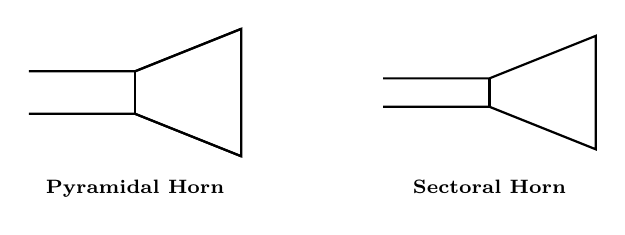
\begin{tikzpicture}[scale=0.9, every node/.style={font=\scriptsize}]
  % Pyramidal Horn (flared in both planes)
  \draw[thick] (0,0.3) -- (1.5,0.3) -- (3.0,0.9) -- (3.0,-0.9) -- (1.5,-0.3) -- (0,-0.3);
  \draw[thick] (1.5,0.3) -- (1.5,-0.3);
  \draw[thick] (3.0,0.9) -- (3.0,-0.9);
  \draw[thick] (1.5,0.3) -- (3.0,0.9);
  \draw[thick] (1.5,-0.3) -- (3.0,-0.9);
  \node[below, font=\scriptsize\bfseries] at (1.5,-1.1) {Pyramidal Horn};
  
  % Sectoral Horn
  \draw[thick] (5,0.2) -- (6.5,0.2) -- (8.0,0.8) -- (8.0,-0.8) -- (6.5,-0.2) -- (5,-0.2);
  \draw[thick] (6.5,0.2) -- (6.5,-0.2);
  \node[below, font=\scriptsize\bfseries] at (6.5,-1.1) {Sectoral Horn};
\end{tikzpicture}
\end{tcolorbox}

\textbf{Pyramidal Horn Gain:}
  \begin{equation}
    G = \frac{4\pi}{\lambda^2} \epsilon_{ap} A = \frac{4\pi}{\lambda^2} \epsilon_{ap} (a_e b_e)
  \end{equation}
  where $a_e, b_e$ are the aperture widths and $\epsilon_{ap}$ is the aperture efficiency.

\subsection{Parabolic Reflector Antenna}
Reflector antennas focus a feed horn's spherical wavefronts into highly directive plane waves.
\textbf{Cassegrain Feed:} Uses a primary parabolic reflector, a secondary hyperbolic sub-reflector at the focus, and a feed horn placed at the vertex of the primary dish.

\begin{tcolorbox}[tikzbox, title={Cassegrain Feed Ray-Tracing Geometry}]
\centering
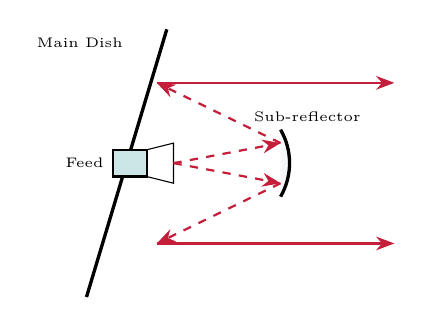
\begin{tikzpicture}[scale=0.85]
  % Main parabolic dish
  \draw[very thick, domain=-2:2, samples=50] plot (\x*0.3 - 0.5, \x);
  
  % Sub-reflector (hyperbolic)
  \draw[very thick, fill=mygray] (1.8,-0.5) arc (-30:30:1.0);
  
  % Feed horn at vertex
  \draw[thick, fill=myteal!20] (-0.7,-0.2) rectangle (-0.2,0.2);
  \draw (-0.2,0.2) -- (0.2,0.3) -- (0.2,-0.3) -- (-0.2,-0.2);
  \node[left, font=\tiny] at (-0.7,0) {Feed};
  
  % Ray tracing (horn -> sub-reflector -> dish -> out)
  \draw[arrow, color=myred, dashed] (0.2,0) -- (1.8,0.3);
  \draw[arrow, color=myred, dashed] (1.8,0.3) -- (-0.05, 1.2);
  \draw[arrow, color=myred] (-0.05, 1.2) -- (3.5, 1.2);
  
  \draw[arrow, color=myred, dashed] (0.2,0) -- (1.8,-0.3);
  \draw[arrow, color=myred, dashed] (1.8,-0.3) -- (-0.05, -1.2);
  \draw[arrow, color=myred] (-0.05, -1.2) -- (3.5, -1.2);
  
  \node[font=\tiny] at (2.2,0.7) {Sub-reflector};
  \node[font=\tiny] at (-1.2,1.8) {Main Dish};
\end{tikzpicture}
\end{tcolorbox}

\textbf{Gain:} $G = \left(\frac{\pi D}{\lambda}\right)^{\!2} \eta_{ap}$ where $D$ is the diameter of the dish.

% ===============================================================================
\section{Airborne and Planar Antennas}
% ===============================================================================

Airborne antennas must be aerodynamic, low-weight, and often conformal (matching the contour of the aircraft skin).

\subsection{Microstrip Patch Antenna}
A microstrip patch antenna consists of a radiating metallic patch printed on one side of a thin dielectric substrate with a continuous ground plane on the other.

\begin{tcolorbox}[tikzbox, title={Microstrip Patch Antenna Structure}]
\centering
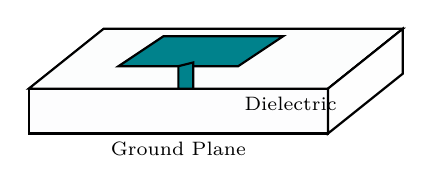
\begin{tikzpicture}[scale=0.95]
  % Substrate (3D-like box)
  \draw[thick, fill=mygray!30] (0,0) -- (4,0) -- (5,0.8) -- (1,0.8) -- cycle;
  \draw[thick, fill=mygray!20] (0,-0.6) -- (4,-0.6) -- (4,0) -- (0,0) -- cycle;
  \draw[thick, fill=mygray!10] (4,-0.6) -- (5,0.2) -- (5,0.8) -- (4,0) -- cycle;
  
  % Patch (printed on top of substrate)
  \draw[thick, fill=myteal] (1.2,0.3) -- (2.8,0.3) -- (3.4,0.7) -- (1.8,0.7) -- cycle;
  
  % Microstrip feed line
  \draw[thick, fill=myteal] (2.0,0) -- (2.0,0.3) -- (2.2,0.35) -- (2.2,0) -- cycle;
  
  % Labels
  \node[font=\scriptsize\color{myteal}] at (2.3,0.5) {Patch};
  \node[font=\scriptsize] at (3.5,-0.2) {Dielectric};
  \node[font=\scriptsize] at (2,-0.8) {Ground Plane};
\end{tikzpicture}
\end{tcolorbox}

\textbf{Feed Techniques:}
\begin{enumerate}[leftmargin=*, itemsep=3pt]
  \item \textbf{Microstrip Line Feed:} Easy to print, easy to match using inset cuts.
  \item \textbf{Coaxial Probe Feed:} Feed probe is connected through a hole from the bottom ground, matching is done by adjusting the insertion point.
  \item \textbf{Aperture-Coupled Feed:} Non-contact feed where a slot in the ground plane couples energy from a bottom line.
  \item \textbf{Proximity-Coupled Feed:} Multi-layer line printed directly below the patch.
\end{enumerate}

% ===============================================================================
% MANDATORY QUICK REVISION PAGE
% ===============================================================================
\newpage
\begin{center}
  {\large\bfseries\color{myred} Quick Revision --- Module VII}\\[3pt]
  {\small\color{mydark} Microwave Antennas $|$ PE-EC701A}
\end{center}
\noindent{\color{myred}\rule{\linewidth}{1.2pt}}
\vspace{4pt}

\begin{tcolorbox}[formulabox, title={\textbf{Key Formulas at a Glance}}]
\renewcommand{\arraystretch}{1.3}
\begin{tabularx}{\linewidth}{B{4.5cm} X}
Effective Aperture      & $A_e = \frac{\lambda^2}{4\pi} G$ \\[4pt]
Horn Antenna Gain       & $G = \frac{4\pi}{\lambda^2} \epsilon_{ap} (a_e b_e)$ \\[4pt]
Parabolic Dish Gain     & $G = \left(\frac{\pi D}{\lambda}\right)^{\!2} \eta_{ap}$ \\[4pt]
Parabolic HPBW          & $\text{HPBW} \approx 70 \frac{\lambda}{D} \quad (\text{degrees})$ \\[4pt]
Patch Length            & $L \approx \frac{c}{2 f_0 \sqrt{\epsilon_{\text{eff}}}} - 2\Delta L$
\end{tabularx}
\tcbset{colbacktitle=mygreen, coltitle=white}
\end{tcolorbox}

\begin{tcolorbox}[defbox, title={\textbf{One-Line Definitions}}]
\begin{itemize}[leftmargin=*, itemsep=2.5pt, topsep=0pt]
  \item \textbf{Directivity:} The ratio of maximum radiation intensity to average radiation intensity.
  \item \textbf{Pyramidal Horn:} A waveguide flaring in both electric and magnetic field planes to match free space.
  \item \textbf{Cassegrain Feed:} A dual-reflector antenna utilizing a parabolic dish and a hyperbolic sub-reflector.
  \item \textbf{Aperture Efficiency:} The ratio of the effective antenna aperture to its physical geometric area.
  \item \textbf{Polarization:} The orientation of the electric field vector of the radiated wave as it propagates.
  \item \textbf{Conformal Antenna:} An antenna designed to follow the curved contour of an host aircraft or vehicle.
  \item \textbf{Aperture Coupling:} A non-contact microstrip feeding technique using a slot in a shared ground plane.
\end{itemize}
\end{tcolorbox}

\begin{tcolorbox}[exambox, title={\textbf{Frequently Asked / Viva Questions}}]
\begin{enumerate}[topsep=0pt, label=\textbf{Q\arabic*.}, itemsep=5pt]
  \item \Q{State the relation between antenna gain, directivity, and efficiency.}
    $G = \eta_{\text{rad}} \cdot D$, where $\eta_{\text{rad}}$ is the radiation efficiency. For a lossless antenna, gain equals directivity ($G = D$).
  \item \Q{What are the advantages of Cassegrain feeds over focal-point feeds?}
    Shorter waveguide feed lines (reducing insertion loss), lower spillover noise from the ground, and easier access to the feed horn at the vertex.
  \item \Q{Explain the physical operation of a microstrip patch antenna.}
    The patch acts as a resonant cavity. Radiation occurs primarily from the fringing fields at the open-circuited edges of the patch.
  \item \Q{Why does flaring a waveguide into a horn antenna increase directivity?}
    Flaring increases the physical aperture area of the waveguide. Since $D \propto A/\lambda^2$, a larger aperture yields higher directivity and narrower beamwidth.
  \item \Q{What is circular polarization and when is it preferred?}
    A wave polarization where the E-field vector rotates in a circle. It is preferred in satellite links because it is immune to Faraday rotation in the ionosphere.
  \item \Q{Why do planar antennas require low-profile feed techniques in airborne systems?}
    To maintain aerodynamic properties, preventing wind drag, turbulence, and structural damage to the aircraft.
  \item \Q{State the difference between E-plane and H-plane sectoral horns.}
    An E-plane horn flares only in the direction of the electric field. An H-plane horn flares only in the direction of the magnetic field.
  \item \Q{How does the dielectric substrate thickness affect microstrip patch performance?}
    Thicker substrates increase bandwidth and radiation efficiency but lead to surface-wave excitation, causing radiation pattern degradation.
  \item \Q{What is FNBW and how is it related to HPBW?}
    FNBW is First-Null Beamwidth. For symmetric main lobes, FNBW is approximately twice the HPBW ($\text{FNBW} \approx 2 \times \text{HPBW}$).
  \item \Q{What is the purpose of the sub-reflector in a Cassegrain antenna?}
    To reflect the feed signals onto the main dish, allowing the feed electronics to be placed behind the main dish rather than suspended at the focus.
  \item \Q{How do lens antennas work at microwave frequencies?}
    They use dielectric materials to collimate spherical wavefronts into plane waves, similar to optical lenses.
  \item \Q{What is the typical gain range of a standard horn antenna?}
    Typically between $10\text{ dB}$ and $25\text{ dB}$, depending on flaring and operating frequency.
\end{enumerate}
\tcbset{colbacktitle=mgframe, coltitle=mydark}
\end{tcolorbox}

\begin{tcolorbox}[tikzbox, title={Comparison of Microwave Antennas}]
\renewcommand{\arraystretch}{1.4}
\par\noindent
\begin{tabularx}{\linewidth}{|B{3.0cm}|Y|Y|Y|}
\hline
\rowcolor{hdrgray}
\textbf{Antenna Type} & \textbf{Typical Gain} & \textbf{Bandwidth} & \textbf{Physical Profile} \\
\hline
\textbf{Horn Antenna} & Moderate ($12 - 25$ dBi) & Wide (waveguide range) & Bulky flared structure \\
\hline
\rowcolor{rowalt}
\textbf{Parabolic Dish} & Very High ($30 - 50$ dBi) & Wide & Very bulky reflector assembly \\
\hline
\textbf{Microstrip Patch} & Low ($5 - 8$ dBi) & Very Narrow ($2\% - 5\%$) & Flat, lightweight, conformal \\
\hline
\rowcolor{rowalt}
\textbf{Lens Antenna} & High ($20 - 30$ dBi) & Moderate & Heavy dielectric component \\
\hline
\end{tabularx}
\end{tcolorbox}

\end{document}
